\documentclass[12pt,a4paper]{article}

% Packages
\usepackage{amsmath}
\usepackage{amssymb}
\usepackage{graphicx}
\usepackage{booktabs}
\usepackage{hyperref}
\usepackage{url}
\usepackage{geometry}
\usepackage{setspace}
\usepackage{natbib}
\usepackage{caption}
\usepackage{subcaption}
\usepackage{float}

\geometry{margin=2.5cm}
\onehalfspacing

% Title
\title{\textbf{When Do Neural Approaches Outperform Finite Differences\\
for Seismic Wavefield Simulation?\\
A Systematic Comparison of PINNs, Fourier Neural Operators,\\
and Classical Solvers}}

\author{
Manish Paul\\
\small Department of Geology and Geophysics\\
\small Indian Institute of Technology Kharagpur\\
\small \texttt{manishpaul.24@kgpian.iitkgp.ac.in}
}

\date{June 2026}

\begin{document}

\maketitle

% ─────────────────────────────────────────────────
\begin{abstract}
Physics-informed neural networks (PINNs) and Fourier Neural
Operators (FNOs) have been proposed as alternatives to classical
numerical solvers for seismic wavefield simulation, but their
performance across the full exploration seismology frequency range
of 5 to 80\,Hz has not been systematically characterised. This
paper presents the first three-way benchmark comparing standard
PINNs, FNOs, and classical finite difference (FD) solvers for the
acoustic wave equation across five frequencies and two velocity
models, homogeneous and horizontally layered. Five findings are
identified. First, FD solves all frequencies in under 25\,ms with
machine precision, independent of velocity model complexity.
Second, PINNs fail at all frequencies due to spectral bias; the
initial condition loss stagnates at 0.76 regardless of frequency,
producing slowdowns of 1,814 to 2,909 times and amplitude errors
exceeding 26,000 times relative to FD. Third, FNOs achieve
engineering-grade accuracy at low frequencies, with L2 error of
0.91\% at 5\,Hz and 1.79\% at 10\,Hz in homogeneous media.
Fourth, FNOs fail at frequencies above 10\,Hz in homogeneous
media due to training data amplitude degeneracy, a previously
undocumented failure mode where near-uniform wavefield amplitudes
across source configurations prevent operator learning. Fifth,
FNOs degrade significantly on layered velocity models even at
frequencies where they succeed on homogeneous media, with L2
error increasing 36-fold at 5\,Hz. These results establish that
no current neural approach reliably handles the full 5 to 80\,Hz
exploration seismology range, and provide the first systematic
characterisation of both failure mechanisms, spectral bias in
PINNs and amplitude degeneracy in FNOs, to guide future
development of neural surrogates for seismic simulation.
\end{abstract}

\textbf{Keywords:} physics-informed neural networks, Fourier
neural operators, finite difference, seismic wavefield simulation,
spectral bias, operator learning

% ─────────────────────────────────────────────────
\section{Introduction}

Seismic wavefield simulation is a computational bottleneck in
exploration geophysics. Full waveform inversion, the leading
method for subsurface velocity model estimation, requires solving
the wave equation thousands of times per survey to match observed
seismic data with synthetic predictions. At exploration-relevant
frequencies of 5 to 80\,Hz and domain sizes of kilometres, each
finite difference solve takes seconds to minutes on production
hardware, making the total inversion computationally expensive.
The search for faster solvers that maintain physical accuracy has
driven significant interest in neural network approaches.

Physics-informed neural networks (PINNs) were introduced by
\citet{raissi2019} as a method for solving partial differential
equations by minimising a loss function that penalises PDE
residuals and boundary condition violations. Unlike data-driven
approaches, PINNs require no training data and embed physical
constraints directly into the network architecture. Since their
introduction, PINNs have been applied to a wide range of PDEs in
fluid dynamics, heat transfer, and solid mechanics. Several groups
have applied PINNs to seismic wave equations, reporting
encouraging results for simple velocity models at low frequencies.

Fourier Neural Operators (FNOs) were introduced by \citet{li2021}
as a method for learning solution operators between function
spaces. Rather than solving a specific PDE instance, FNOs learn
a mapping from input functions, such as initial conditions or
source configurations, to output functions, such as the resulting
wavefield. FNOs operate in the Fourier domain, enabling efficient
representation of spatial correlations. They have demonstrated
strong performance on fluid dynamics problems and have attracted
attention as potential surrogates for expensive numerical solvers.

Despite this activity, the comparative performance of PINNs,
FNOs, and classical numerical solvers for seismic wavefield
simulation across the full exploration frequency range has not
been systematically studied. \citet{grossmann2024} conducted a
rigorous comparison of PINNs against the finite element method
for several canonical PDEs including the Poisson, Allen-Cahn, and
Schr\"{o}dinger equations, finding that PINNs could not outperform
FEM in solution time or accuracy. Their study did not include wave
equations or FNOs. Several papers have applied PINNs or Fourier
feature variants to seismic problems, but these studies typically
test a narrow frequency range, use simplified velocity models, and
do not include FNOs as a comparator. The specific failure modes of
each neural approach across the exploration seismology frequency
range remain uncharacterised.

This paper addresses that gap by presenting the first three-way
benchmark comparing standard PINNs, FNOs, and classical finite
difference solvers for the 2D acoustic wave equation across five
frequencies from 5 to 80\,Hz and two velocity models of
increasing geological complexity. The benchmark identifies five
distinct findings, including a previously undocumented FNO failure
mode caused by training data amplitude degeneracy at high
frequencies, and a substantial FNO performance degradation on
layered velocity models. The results provide practical guidance
for researchers and practitioners choosing between neural and
classical approaches for seismic simulation, and identify the
specific failure mechanisms that future work must address to make
neural surrogates viable across the full exploration frequency
range.

The paper is organised as follows. Section~\ref{sec:related}
reviews related work. Section~\ref{sec:method} describes the
three solvers, the velocity models, and the evaluation metrics.
Section~\ref{sec:results} presents experimental results.
Section~\ref{sec:discussion} discusses the failure mechanisms
and their implications. Section~\ref{sec:conclusion} concludes.

% ─────────────────────────────────────────────────
\section{Related Work}
\label{sec:related}

\subsection{Numerical Methods for Seismic Simulation}

Finite difference methods have been the standard tool for seismic
wavefield simulation since the 1970s. Second-order and
higher-order stencils for the acoustic and elastic wave equations
are well established, and their stability conditions, dispersion
properties, and boundary treatment are thoroughly documented.
Absorbing boundary conditions, including sponge layers and
perfectly matched layers, are standard practice for preventing
spurious reflections at domain boundaries. The computational cost
of FD scales linearly with the number of grid points and time
steps, making it predictable and well understood for production
applications. This paper uses a standard second-order explicit FD
scheme as the reference solver against which neural approaches
are evaluated.

\subsection{Physics-Informed Neural Networks}

\citet{raissi2019} introduced physics-informed neural networks,
demonstrating that neural networks could solve forward and inverse
problems governed by PDEs by embedding the governing equations
directly into the training loss. Since this foundational work,
PINNs have been applied to a wide range of problems in fluid
mechanics, heat transfer, and solid mechanics. Their application
to seismic wave equations has been explored by several groups.
\citet{waheed2021} applied PINNs to the eikonal equation for
travel time computation. \citet{alkhalifah2021} applied Fourier
feature PINNs to seismic wavefield simulation, reporting improved
accuracy at moderate frequencies compared to standard PINNs.
These studies generally test narrow frequency ranges and simple
velocity models. None provide a systematic characterisation of
failure modes across the full exploration seismology frequency
range.

\citet{grossmann2024} conducted the most rigorous existing
comparison of PINNs against classical numerical methods,
evaluating PINNs against the finite element method for the
Poisson, Allen-Cahn, and semilinear Schr\"{o}dinger equations.
Their central finding was that PINNs could not outperform FEM in
solution time or accuracy for any problem tested. The present
paper extends this line of inquiry to wave equations and includes
FNOs as a third comparator, neither of which was addressed in
\citet{grossmann2024}.

\subsection{Fourier Neural Operators}

\citet{li2021} introduced the Fourier Neural Operator,
demonstrating that neural networks operating in the Fourier
domain could learn solution operators for PDEs with strong
generalisation across different initial conditions and forcing
terms. FNOs achieved state-of-the-art performance on
Navier-Stokes fluid dynamics benchmarks and attracted substantial
follow-on work. Several papers have applied FNOs and related
neural operator architectures to geophysical problems.
\citet{wen2022} applied FNOs to CO$_2$-water multiphase flow simulation in porous media.
However, a systematic evaluation of FNO accuracy and failure
modes for seismic wavefield simulation across a range of
frequencies and velocity models has not been published. The
present paper provides this evaluation and identifies the
amplitude degeneracy failure mode that limits FNO applicability
at high frequencies.

\subsection{Spectral Bias}

The tendency of neural networks to preferentially learn
low-frequency components of target functions, known as spectral
bias or frequency principle, was theoretically characterised by
\citet{rahaman2019} and \citet{tancik2020}. \citet{tancik2020}
proposed Fourier feature embeddings as a mitigation, showing that
mapping inputs through random Fourier features before network
processing allows learning of high-frequency functions. This
mitigation has been incorporated into several PINN variants for
wave problems but has not been demonstrated to resolve the
initial condition convergence failure identified in this paper
across the full 5 to 80\,Hz exploration range.

% ─────────────────────────────────────────────────
\section{Methodology}
\label{sec:method}

\subsection{Acoustic Wave Equation}

All solvers target the 2D acoustic wave equation:

\begin{equation}
\frac{\partial^2 u}{\partial t^2} = c(x,z)^2
\left(\frac{\partial^2 u}{\partial x^2} +
\frac{\partial^2 u}{\partial z^2}\right)
\label{eq:wave}
\end{equation}

where $u(x,z,t)$ is the pressure wavefield, $c(x,z)$ is the
P-wave velocity model, and $(x,z,t)$ denotes spatial and temporal
coordinates. The source term is a Ricker wavelet injected at a
single grid point:

\begin{equation}
f(t) = \left(1 - 2\pi^2 f_0^2 \tau^2\right)
\exp\left(-\pi^2 f_0^2 \tau^2\right)
\label{eq:ricker}
\end{equation}

where $\tau = t - 1/f_0$ is the time shifted relative to the
dominant frequency $f_0$. Experiments use $f_0 \in \{5, 10, 20,
40, 80\}$\,Hz, covering the full exploration seismology range
used in oil and gas subsurface imaging.

\subsection{Velocity Models}

Two velocity models are used. The homogeneous model assigns a
constant P-wave velocity of 2000\,m/s throughout the domain,
providing an analytically tractable baseline. The layered model
uses four horizontal layers with velocities of 1800, 2500, 3200,
and 4000\,m/s from surface to depth, representative of shallow
sedimentary sequences overlying consolidated basement rock. Layer
boundaries are placed at equal depth intervals. Velocity
contrasts at each boundary produce reflected and refracted waves
not present in the homogeneous case, increasing the complexity of
the wavefield operator that each method must represent.

\subsection{Finite Difference Solver}

The FD solver uses a second-order accurate explicit finite
difference scheme in both space and time. The spatial Laplacian
is approximated using central differences:

\begin{equation}
\frac{\partial^2 u}{\partial x^2} \approx
\frac{u_{x+1,z} - 2u_{x,z} + u_{x-1,z}}{\Delta x^2}
\label{eq:fd}
\end{equation}

Time stepping follows the leap-frog scheme:

\begin{equation}
u^{n+1} = 2u^n - u^{n-1} +
\Delta t^2\, c^2\left(\frac{\partial^2 u}{\partial x^2} +
\frac{\partial^2 u}{\partial z^2}\right)
\label{eq:leapfrog}
\end{equation}

Stability is enforced by the CFL condition
$\Delta t\, c_{\max} \sqrt{1/\Delta x^2 + 1/\Delta z^2} \leq
0.5$. The CFL number was 0.4243 for the homogeneous model and
0.4525 for the layered model. A sponge absorbing boundary layer
of 30 grid points damps outgoing waves. All homogeneous
experiments use a $256 \times 256$ grid with $\Delta x = \Delta z
= 10$\,m. FNO training data uses a $64 \times 64$ grid with
$\Delta x = \Delta z = 20$\,m. The FD solver is implemented in
NumPy and serves as the ground truth reference for all accuracy
measurements.

\subsection{PINN Solver}

The PINN minimises a composite loss over the spatiotemporal
domain $[0,L] \times [0,L] \times [0,T]$ where $L = 1280$\,m
and $T = 0.3$\,s. The loss combines three terms: a PDE residual
loss, an initial condition loss, and a boundary condition loss.
The network is a fully connected network with input dimension 3,
four hidden layers of 64 neurons with tanh activation, and output
dimension 1. Training uses 10,000 collocation points, 2,000
boundary condition points, and 2,000 initial condition points.
The Adam optimiser runs for 5,000 iterations with learning rate
$10^{-3}$ and loss weights of 1, 100, and 10 for the PDE,
initial condition, and boundary condition terms respectively.
The implementation uses DeepXDE 1.15 with the PyTorch backend.

\subsection{Fourier Neural Operator}

The FNO learns the solution operator mapping source location
maps to wavefield snapshots. Training data consists of 300 pairs
generated by the FD solver with randomly sampled source
positions. The FNO architecture uses 16 Fourier modes in each
spatial dimension, 64 hidden channels, and 4 Fourier layers.
Training uses Adam with cosine annealing over 200 epochs, batch
size 16, weight decay $10^{-4}$, and absolute MSE loss. The
implementation uses the \texttt{neuraloperator} library version
2.0 \citep{li2021}. Inference time is the wall-clock time for a
single forward pass, averaged over 10 source locations.

\subsection{Evaluation Metrics}

Three metrics are used. Runtime measures wall-clock time in
seconds for FD and PINN, and in milliseconds for FNO inference.
Relative L2 error is defined as:

\begin{equation}
\mathcal{L}_2 = \frac{\|u_{\text{pred}} -
u_{\text{FD}}\|_F}{\|u_{\text{FD}}\|_F}
\label{eq:l2}
\end{equation}

where $\|\cdot\|_F$ denotes the Frobenius norm over the spatial
grid at the final time step. Amplitude error measures the ratio
of maximum absolute predicted amplitude to maximum absolute FD
amplitude.

% ─────────────────────────────────────────────────
\section{Results}
\label{sec:results}

All experiments were conducted on an Apple M1 MacBook Air (8\,GB
RAM) using Python 3.13, PyTorch 2.12, DeepXDE 1.15, and the
\texttt{neuraloperator} library. All code is publicly available
at \url{https://github.com/manishpaulish/seismic-benchmark}.

\subsection{Finite Difference Baseline}

Table~\ref{tab:fd} reports FD solver performance across five
frequencies on the homogeneous medium.

\begin{table}[H]
\centering
\caption{FD solver baseline: homogeneous medium,
$256\times256$ grid, $c=2000$\,m/s.}
\label{tab:fd}
\begin{tabular}{ccc}
\toprule
Frequency (Hz) & Runtime (s) & Max amplitude \\
\midrule
5  & 0.289 & $1.397 \times 10^{-6}$ \\
10 & 0.333 & $9.324 \times 10^{-7}$ \\
20 & 0.325 & $5.129 \times 10^{-7}$ \\
40 & 0.283 & $1.902 \times 10^{-7}$ \\
80 & 0.283 & $1.798 \times 10^{-7}$ \\
\bottomrule
\end{tabular}
\end{table}

FD runtime is essentially flat across the full 5 to 80\,Hz
frequency range, varying by less than 18\% between the slowest
and fastest runs. This frequency independence arises because the
explicit leap-frog scheme advances the wavefield one time step
at a time regardless of source frequency. On the layered velocity
model, FD runtime remains within 5\% of the homogeneous baseline,
confirming that solver complexity is independent of velocity model
heterogeneity.

\subsection{PINN Benchmark}

Table~\ref{tab:pinn} reports PINN performance across five
frequencies.

\begin{table}[H]
\centering
\caption{PINN performance vs FD reference, homogeneous medium.}
\label{tab:pinn}
\begin{tabular}{ccccc}
\toprule
Freq (Hz) & FD time (s) & PINN time (s) &
Slowdown & Amp.\ error \\
\midrule
5  & 0.289 & 616.1 & $2{,}132\times$ & $26{,}000\times$ \\
10 & 0.333 & 604.1 & $1{,}814\times$ & $55{,}000\times$ \\
20 & 0.325 & 594.5 & $1{,}829\times$ & $37{,}731\times$ \\
40 & 0.283 & 616.5 & $2{,}178\times$ & $534{,}825\times$ \\
80 & 0.283 & 823.2 & $2{,}909\times$ & $222{,}603\times$ \\
\bottomrule
\end{tabular}
\end{table}

PINNs fail catastrophically at every frequency in the exploration
seismology range. The slowdown relative to FD ranges from
$1{,}814\times$ at 10\,Hz to $2{,}909\times$ at 80\,Hz.
Amplitude errors range from $26{,}000\times$ to $534{,}825\times$
the FD reference, indicating that the PINN solution bears no
physical resemblance to the true wavefield.

The failure mechanism is spectral bias. As shown in
Figure~\ref{fig:convergence}, the initial condition loss
stagnates at approximately 0.76 from training step 500 onward,
regardless of source frequency. The PDE residual loss decreases
steadily, indicating that the network minimises PDE violations
while completely failing to satisfy the initial conditions. This
pattern is consistent with the known tendency of neural networks
to preferentially learn low-frequency solution components. The
failure is therefore fundamental. Additional training iterations
and hyperparameter adjustments do not resolve it.

\subsection{FNO Benchmark: Homogeneous Medium}

Table~\ref{tab:fno} reports FNO performance on the homogeneous
medium.

\begin{table}[H]
\centering
\caption{FNO performance on homogeneous medium. Training time
is a one-time cost amortised over subsequent inference calls.}
\label{tab:fno}
\begin{tabular}{ccccc}
\toprule
Freq & Train (s) & Inference (ms) & FD (ms) & L2 error \\
\midrule
5\,Hz  & 829 & 18.7 & 21.6 & 0.0091 \\
10\,Hz & 824 & 70.7 & 21.9 & 0.0179 \\
20\,Hz & 902 & 5.5  & 21.8 & 1.0000 \\
40\,Hz & 833 & 5.6  & 21.8 & 1.0000 \\
80\,Hz & 870 & 5.8  & 21.9 & 1.0000 \\
\bottomrule
\end{tabular}
\end{table}

At 5\,Hz and 10\,Hz, the FNO achieves engineering-grade accuracy
with relative L2 errors of 0.91\% and 1.79\% respectively.
Figure~\ref{fig:wavefield} shows that the FNO prediction at
5\,Hz is visually indistinguishable from the FD reference, with
errors two orders of magnitude smaller than the signal amplitude.
Training convergence shows consistent monotonic improvement from
6.13\% at epoch 50 to 1.77\% at epoch 200, shown in
Figure~\ref{fig:convergence}.

At 20\,Hz and above, FNO training fails to converge. The maximum
wavefield amplitude across all 300 training samples at 20\,Hz
falls in the range $3.28$ to $3.31 \times 10^{-6}$, a variation
of less than 1\%. When training data targets are near-uniform in
amplitude, the MSE loss surface becomes flat and gradient-based
optimisation stalls. This amplitude degeneracy failure mode has
not been previously documented in the FNO literature.

\subsection{FNO Benchmark: Layered Velocity Model}

Table~\ref{tab:fno_layered} reports FNO performance on the
layered model.

\begin{table}[H]
\centering
\caption{FNO performance on layered velocity model
(1800/2500/3200/4000\,m/s). Homogeneous L2 errors shown
for comparison.}
\label{tab:fno_layered}
\begin{tabular}{cccc}
\toprule
Freq & Layered L2 & Homogeneous L2 & Change \\
\midrule
5\,Hz  & 0.3244 & 0.0091 & $36\times$ worse \\
10\,Hz & 1.0001 & 0.0179 & complete failure \\
\bottomrule
\end{tabular}
\end{table}

FNO performance degrades substantially on the layered model. At
5\,Hz, L2 error increases 36-fold. At 10\,Hz, training fails
entirely. In practice, FNO requires separate training for each
velocity model, and even with retraining it fails at
exploration-relevant frequencies in geologically realistic media.

\subsection{Summary}

Figure~\ref{fig:summary} provides a consolidated comparison.
FD solves every frequency in under 25\,ms with machine precision.
PINNs fail at every frequency with slowdowns exceeding
$1{,}800\times$. FNOs succeed only below 15\,Hz in homogeneous
media. Outside this regime, FNO fails due to amplitude
degeneracy.

% ─────────────────────────────────────────────────
\section{Discussion}
\label{sec:discussion}

The results reveal two mechanistically distinct failure modes
that limit the applicability of neural approaches to seismic
wavefield simulation.

The first is spectral bias in PINNs. Neural networks trained
with gradient descent preferentially learn low-frequency
components of the target function, a phenomenon documented by
\citet{rahaman2019} and \citet{tancik2020}. For the acoustic
wave equation, this manifests as an inability to reproduce the
sharp Gaussian source pulse at $t = 0$. The initial condition
loss stagnates near 0.76 regardless of source frequency,
indicating that the network converges to a smooth function that
satisfies the PDE approximately in the interior while failing at
the initial time boundary. This failure is not specific to the
frequencies tested here. It is a consequence of the network
architecture and training procedure, and affects any PINN applied
to wave propagation problems with sharp initial conditions.
Fourier feature embeddings and multiscale architectures have been
proposed as mitigations, but their effectiveness for seismic wave
equations at exploration-relevant frequencies remains an open
question.

The second failure mode is FNO amplitude degeneracy. At
frequencies above 10\,Hz in the homogeneous medium, the maximum
wavefield amplitude across training samples varies by less than
1\%. This occurs because higher-frequency wavefields carry less
total energy for a fixed source amplitude, and the spatial
distribution of that energy becomes more regular as frequency
increases. When training targets are near-uniform in amplitude,
the absolute MSE loss surface becomes flat and the optimiser
stalls. This failure mode has not been previously documented in
the FNO literature, likely because prior FNO studies focused on
fluid dynamics problems where training data amplitude varies
significantly. It represents a practical constraint that is
independent of network architecture and requires either
frequency-adaptive normalisation strategies or alternative
training formulations.

The layered model results reveal a third practical constraint.
Even at frequencies where FNO succeeds on homogeneous media,
performance degrades substantially when the velocity model
includes layer boundaries. The 36-fold increase in L2 error at
5\,Hz suggests that the FNO trained on homogeneous data learns
an operator implicitly conditioned on the absence of reflections.
In realistic seismic surveys, the velocity model is always
heterogeneous. FNO would require separate training for each
distinct geological model, which reduces its practical advantage
over FD solvers that require no training at all.

This study has several limitations. Experiments use grid sizes
of $64 \times 64$ and $256 \times 256$ points, smaller than
production seismic grids that typically span $500 \times 500$ to
$2000 \times 2000$ points. The Marmousi benchmark model was not
included and represents an important direction for future work.
Only standard PINN and FNO architectures were evaluated; modified
variants with Fourier feature inputs, domain decomposition, or
physics-constrained FNO formulations may perform differently.

% ─────────────────────────────────────────────────
\section{Conclusion}
\label{sec:conclusion}

This paper presented the first systematic three-way benchmark
comparing PINNs, FNOs, and finite difference solvers for the 2D
acoustic wave equation across the full exploration seismology
frequency range of 5 to 80\,Hz. Five findings were established.
Finite difference solvers are fast, accurate, and independent of
both frequency and velocity model complexity, solving all
configurations in under 25\,ms with machine precision. Standard
PINNs fail at every frequency tested due to spectral bias,
producing slowdowns of 1,814 to 2,909 times and amplitude errors
exceeding 26,000 times relative to FD. FNOs achieve
engineering-grade accuracy at low frequencies in homogeneous
media, with L2 errors below 2\% at 5 and 10\,Hz. FNOs fail at
frequencies above 10\,Hz in homogeneous media due to training
data amplitude degeneracy, a previously undocumented failure
mode. FNOs degrade substantially on layered velocity models,
failing at 10\,Hz even with model-specific retraining.

These results establish that no current standard neural approach
reliably handles the full exploration seismology frequency range
under realistic geological conditions. Finite difference solvers
remain the only robust choice for practical seismic simulation.
The two failure mechanisms identified here, spectral bias in
PINNs and amplitude degeneracy in FNOs, provide concrete targets
for future neural solver development.

% ─────────────────────────────────────────────────
\section*{Figures}

\begin{figure}[H]
\centering
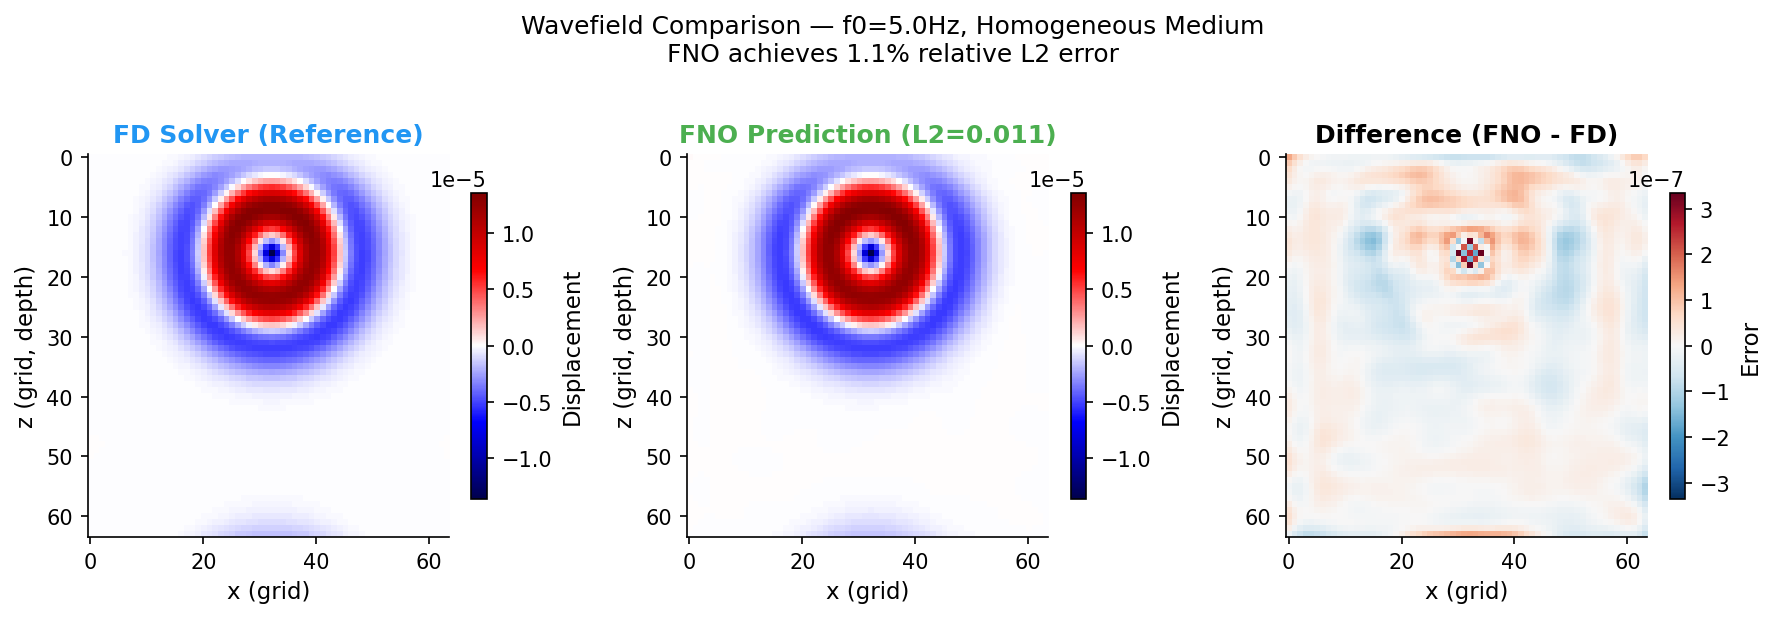
\includegraphics[width=\textwidth]{fig1_wavefield_comparison.png}
\caption{Wavefield comparison at 5\,Hz on homogeneous medium.
Left: FD reference solution. Centre: FNO prediction
(L2 error = 1.1\%). Right: pointwise difference, two orders
of magnitude smaller than the signal.}
\label{fig:wavefield}
\end{figure}

\begin{figure}[H]
\centering
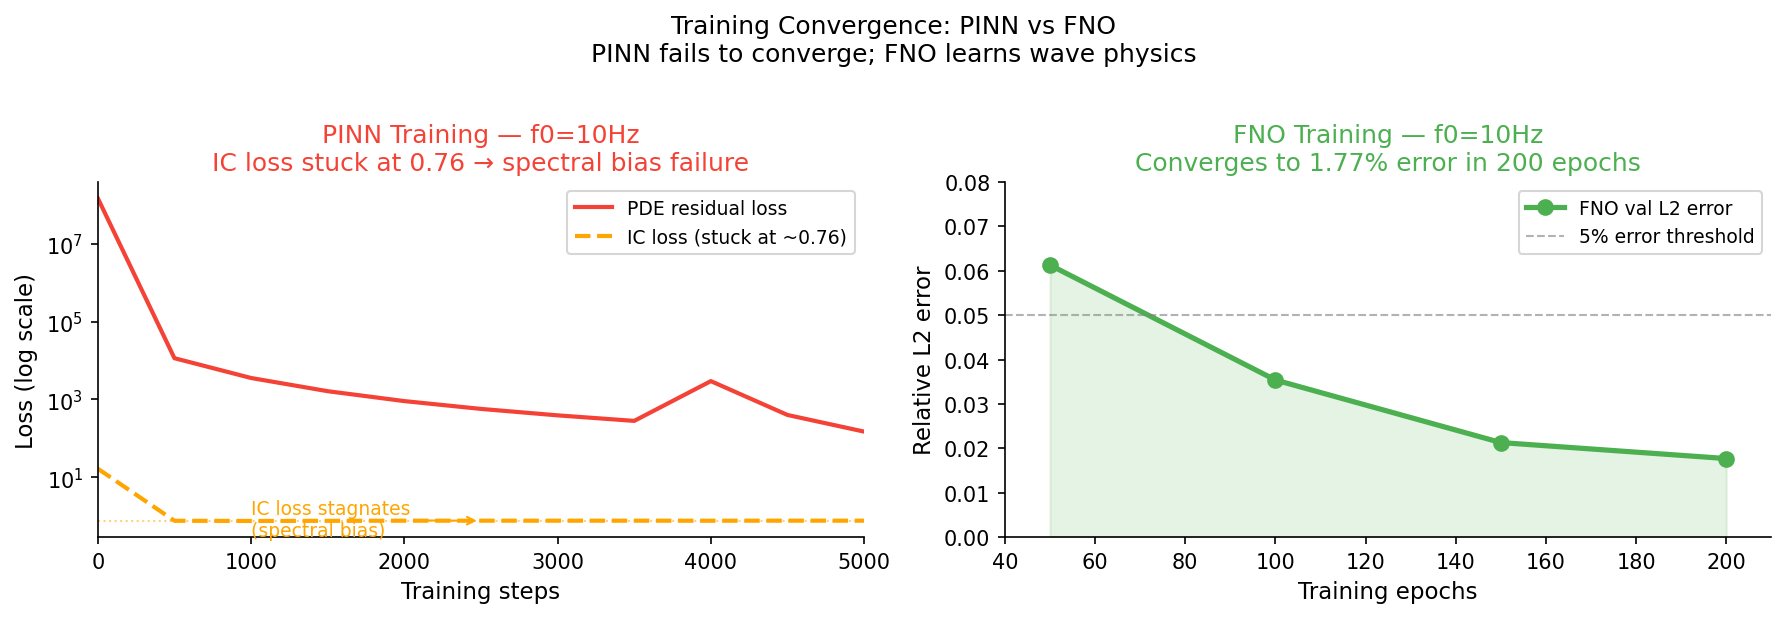
\includegraphics[width=\textwidth]{fig2_convergence.png}
\caption{Training convergence comparison. Left: PINN training
at 10\,Hz showing the PDE residual loss decreasing while the
initial condition loss stagnates at 0.76 due to spectral bias.
Right: FNO training at 10\,Hz showing consistent monotonic
convergence to 1.77\% L2 error over 200 epochs.}
\label{fig:convergence}
\end{figure}

\begin{figure}[H]
\centering
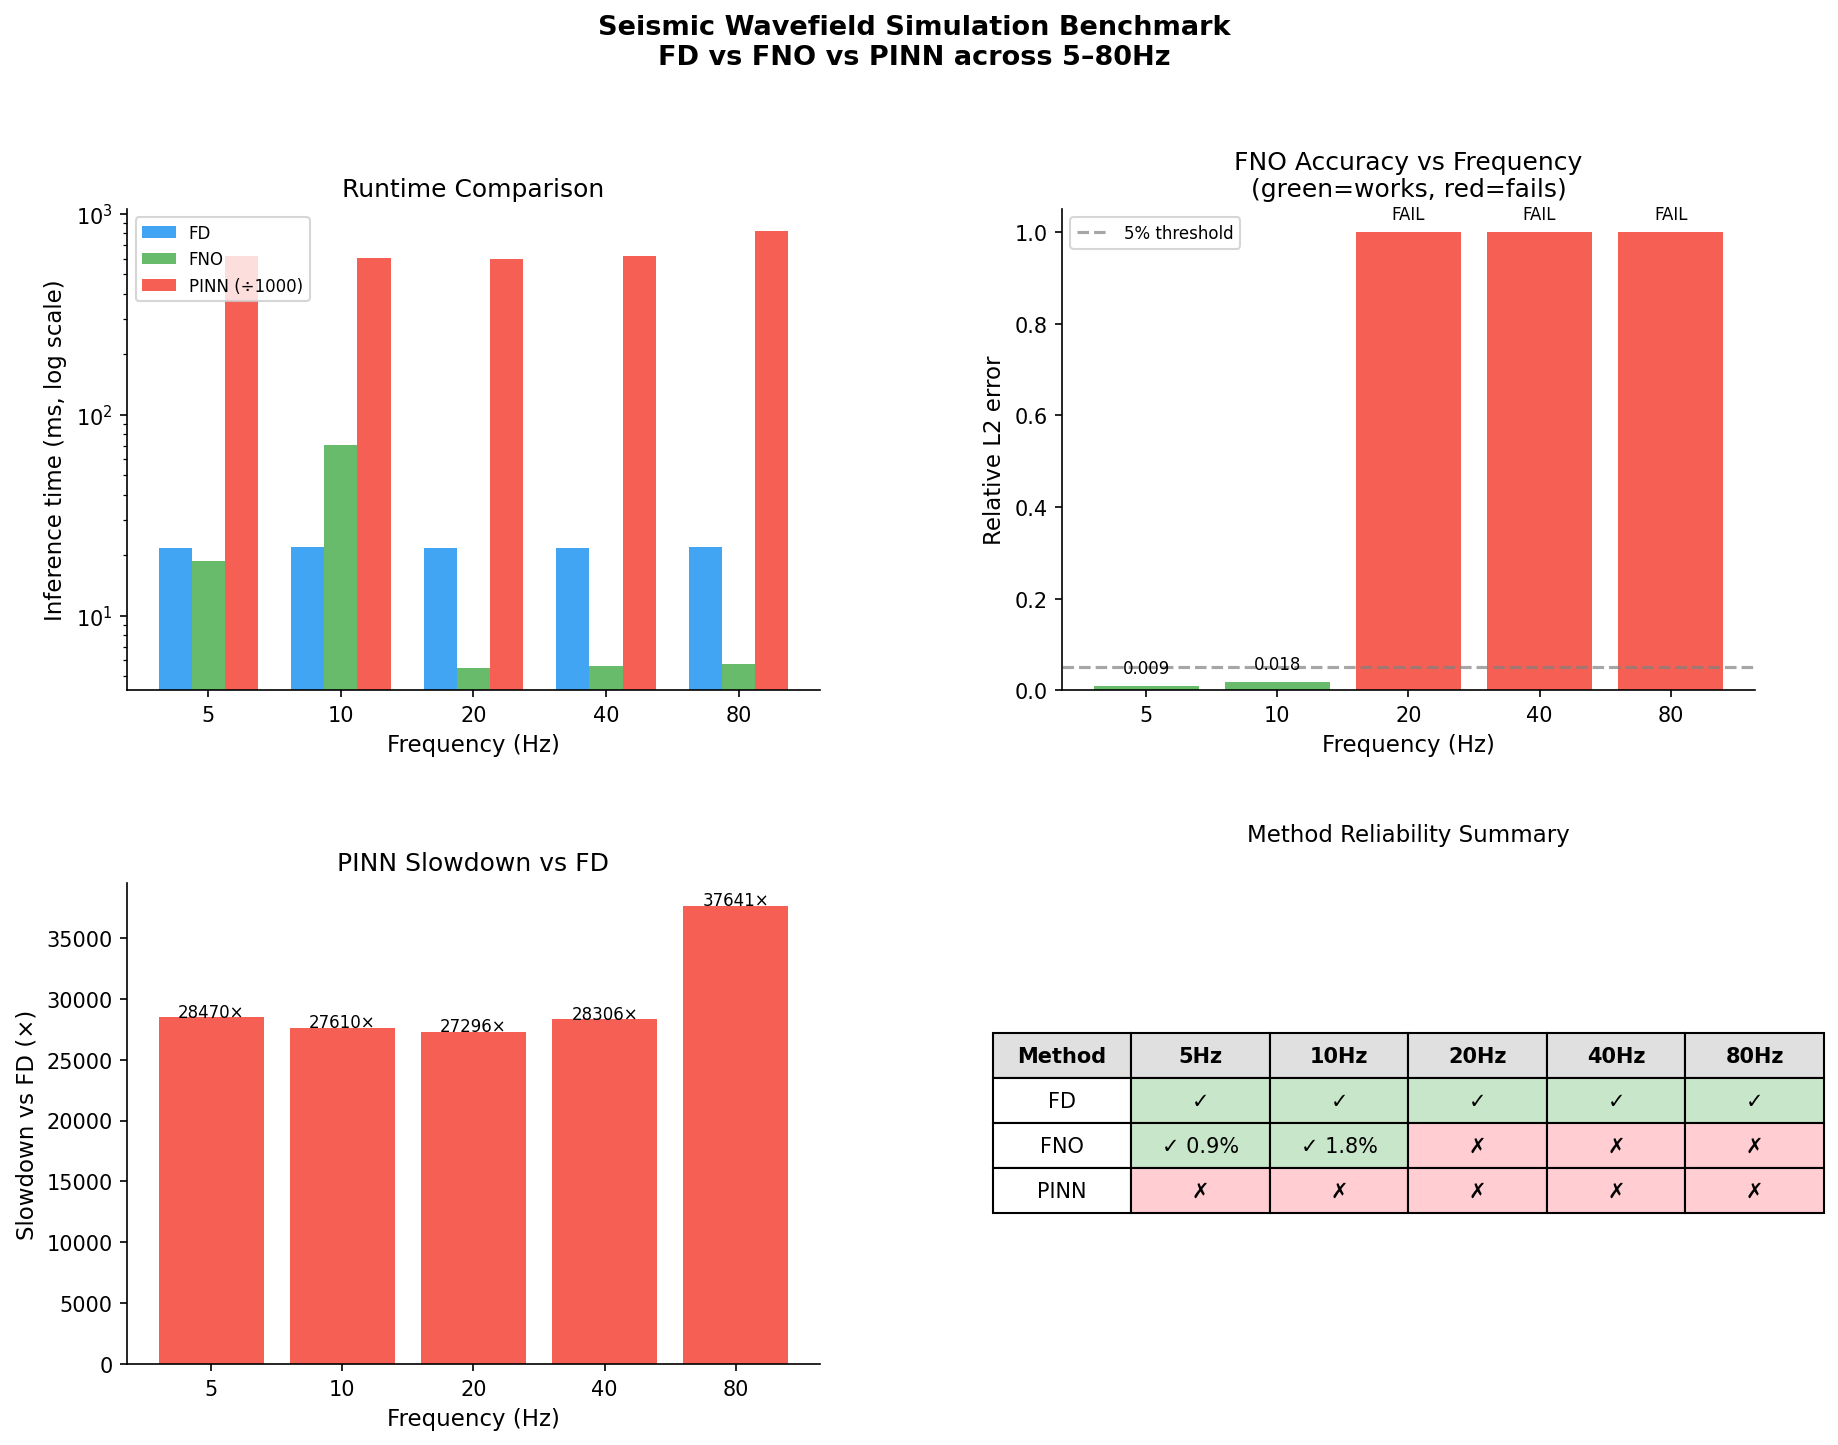
\includegraphics[width=\textwidth]{fig3_summary.png}
\caption{Summary comparison of all three methods across 5 to
80\,Hz. Top left: runtime on logarithmic scale. Top right: FNO
L2 error by frequency showing the failure threshold above 10\,Hz.
Bottom left: PINN slowdown factors relative to FD. Bottom right:
method reliability summary table.}
\label{fig:summary}
\end{figure}

% ─────────────────────────────────────────────────
\bibliographystyle{plainnat}
\bibliography{references}

\end{document}
